\chapter{Problem Description}

\section{Problem Context}
Video people counting asks a system to estimate how many people appear in each frame of a video. This problem is useful in crowd monitoring, classroom analytics, transportation observation, safety systems, and other camera-based applications where the number of people changes over time. In this report, people counting is implemented as an object-detection problem: a detector predicts person bounding boxes, and the final count for a frame is the number of accepted person boxes after post-processing.

The computational challenge comes from repeated CNN inference. A single YOLO inference may be manageable, but a video contains hundreds or thousands of frames, and each frame may be split into several regions to expose more parallel work. The total workload therefore grows with both the number of frames and the number of tiles per frame. This makes the application a good parallel-programming problem: it contains many independent inference calls, but the final counting step still requires careful global merging.

The project focuses on inference rather than training. The YOLO model is fixed and pretrained; the report does not modify model weights or propose a new detector. The technical problem is to build a distributed-memory runtime that executes the same inference pipeline faster on multiple MPI ranks while preserving the output of the corresponding serial pipeline.

\section{YOLO Video People Counting}
The input is a finite video sequence:
\begin{equation}
    V = \{F_1, F_2, \ldots, F_N\}.
\end{equation}
For each frame \(F_i\), the detector produces a set of candidate person detections. Each detection contains a bounding box, a confidence score, and a class label. After filtering and duplicate removal, the target output is the number of final person boxes:
\begin{equation}
    count(F_i) = |\{b \mid b \text{ is a final person bounding box in } F_i\}|.
\end{equation}
The full output of the pipeline is therefore a sequence of frame-level counts:
\begin{equation}
    C = \{count(F_1), count(F_2), \ldots, count(F_N)\}.
\end{equation}

The detector backend is a pretrained YOLO11n model executed through a local Python worker process \cite{ultralytics2026}. YOLO11 follows the usual one-stage detector structure with a feature-extraction backbone, a feature-fusion neck, and multi-scale detection heads, as shown in Figure~\ref{fig:yolo11-architecture}. In this project, YOLO is treated as a detector backend. The MPI program does not split individual neural-network layers or kernels; instead, it distributes repeated YOLO calls across independent video regions.

\begin{figure}[H]
\centering
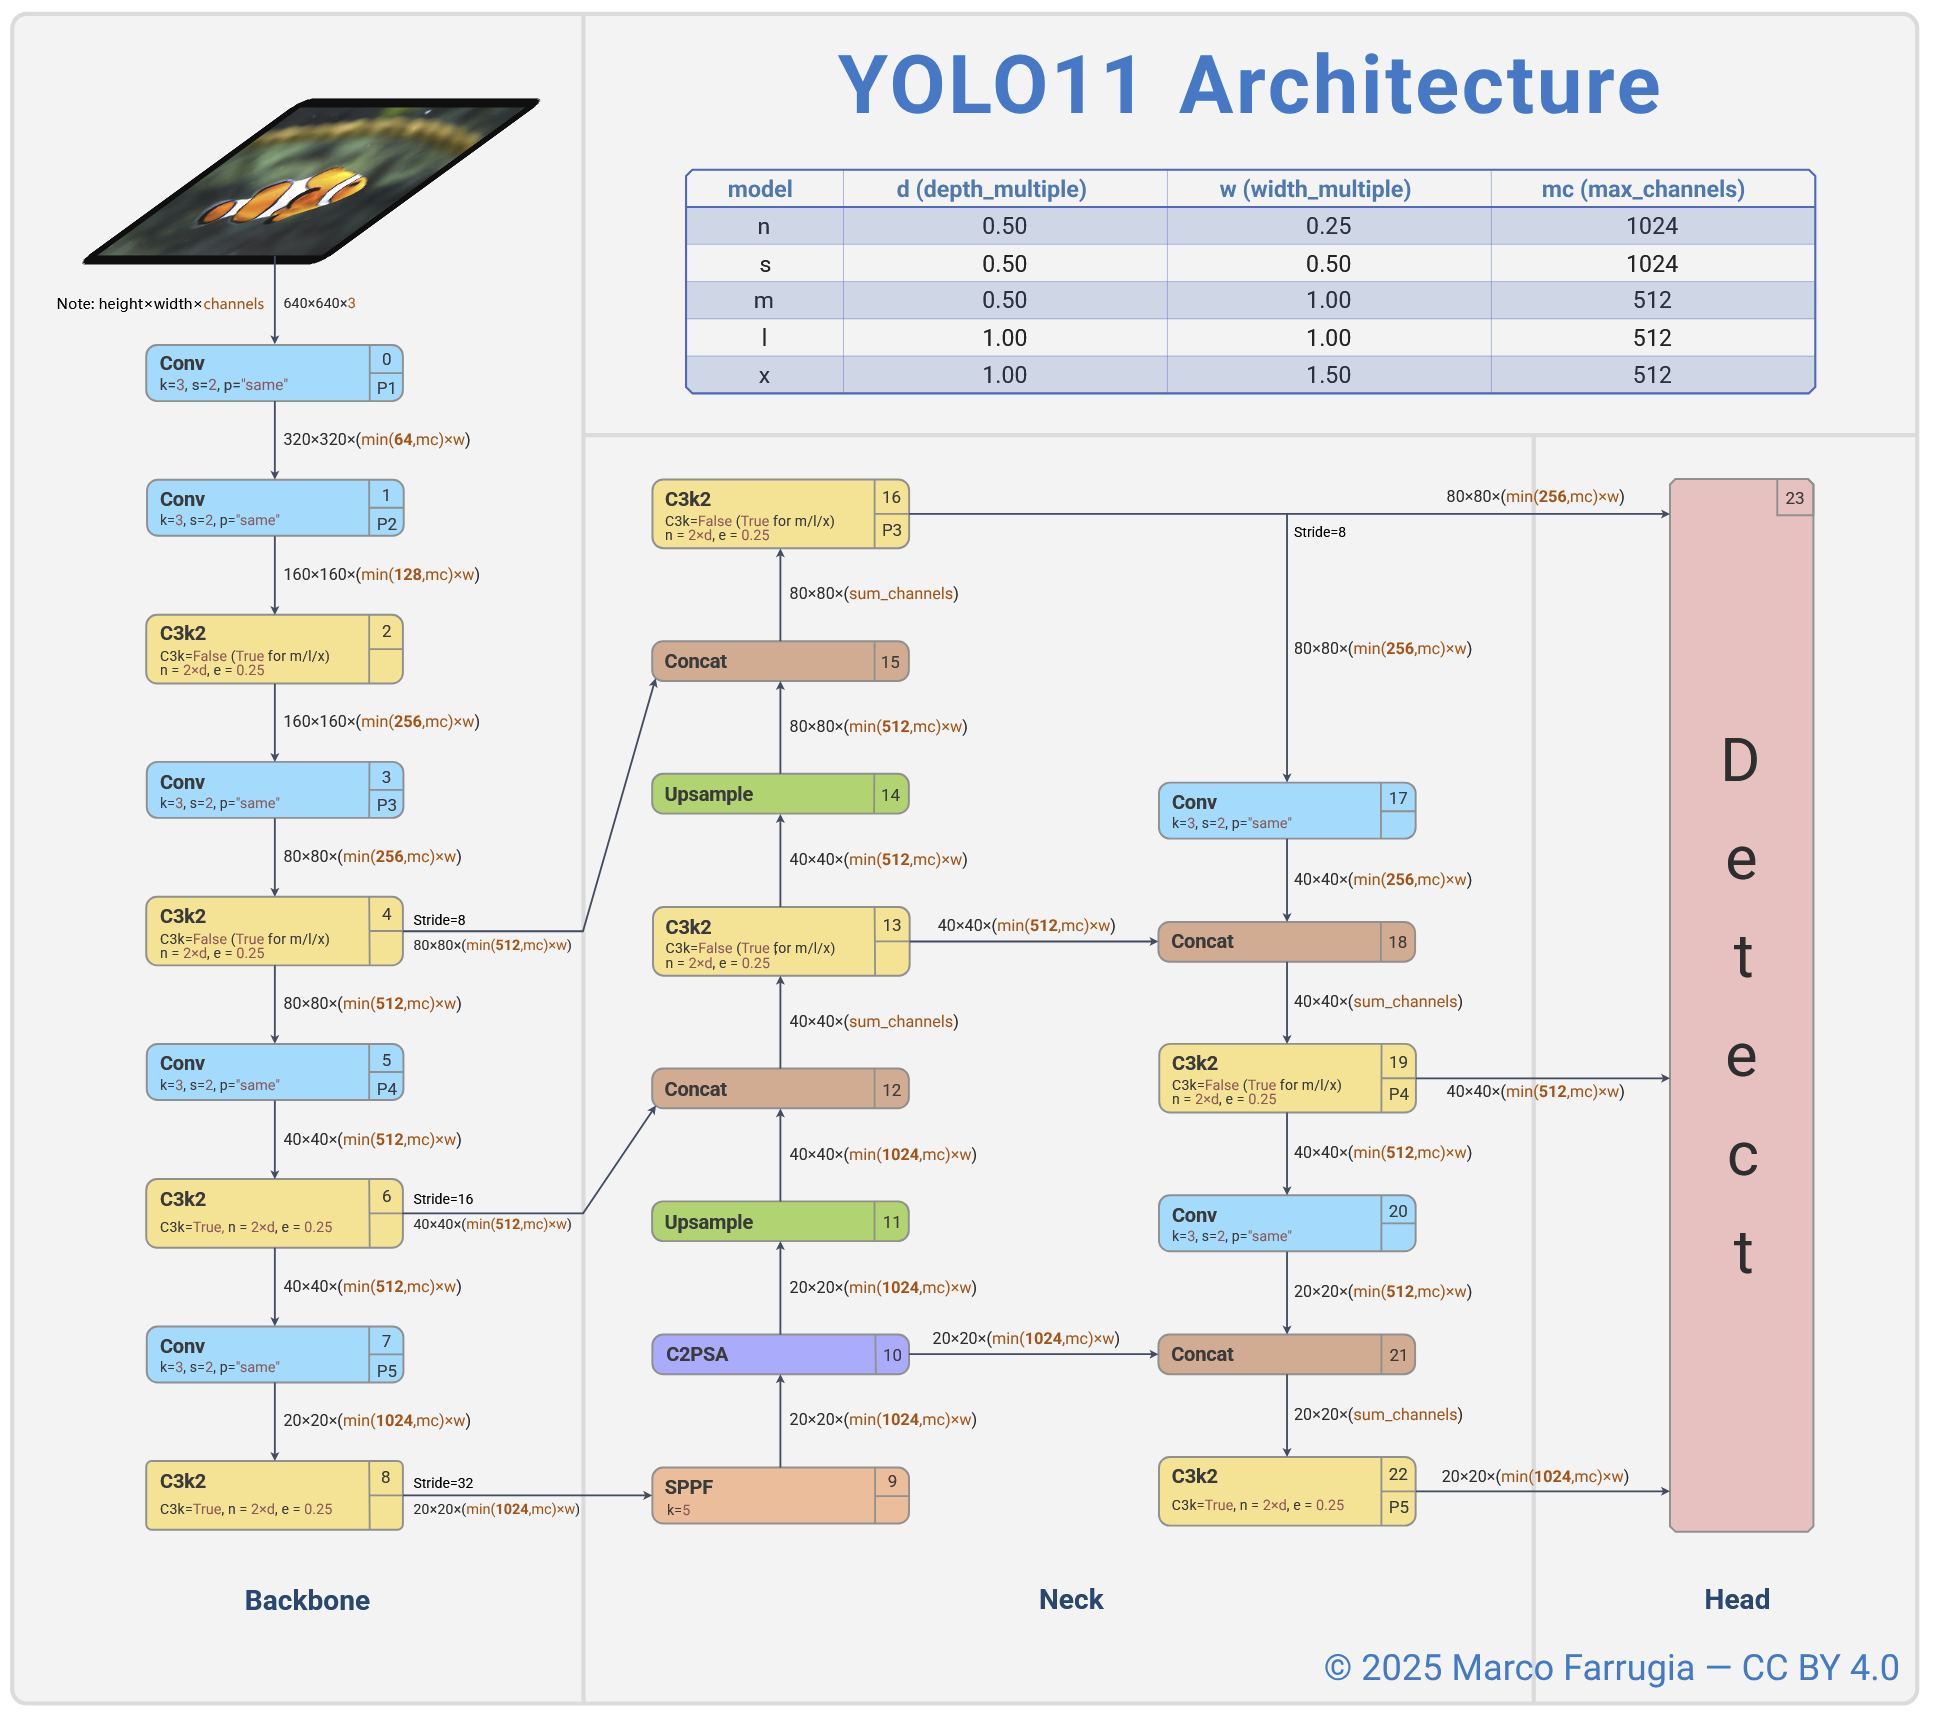
\includegraphics[width=0.95\textwidth]{figures/yolo11_architecture.png}
\caption{YOLO11 object-detection architecture used as the detector backend in this project. Source: Farrugia, CC BY 4.0, Zenodo DOI 10.5281/zenodo.17508018 \cite{farrugia2025yolo11diagram}.}
\label{fig:yolo11-architecture}
\end{figure}

\section{Temporal-Spatial Task Definition}
Frame-only parallelism is possible because frames are naturally ordered but mostly independent for this counting task. However, if only complete frames are distributed, the number of tasks may be too small to keep many MPI ranks busy, especially for short videos or small experiments. The project therefore uses a hybrid decomposition: each video is split by time into frames, and each frame is split by space into image tiles.

For a tile grid with \(R\) rows and \(C\) columns, frame \(F_i\) is decomposed into:
\begin{equation}
    F_i \rightarrow \{T_{i,1}, T_{i,2}, \ldots, T_{i,R \times C}\}.
\end{equation}
A parallel task is one YOLO inference on one frame-tile pair:
\begin{equation}
    task(i,j) = T_{i,j}, \qquad |\mathcal{T}| = N \times R \times C.
\end{equation}
This definition turns video inference into a task-parallel workload. Larger values of \(R\) and \(C\) create more tasks, which can improve utilization and load balancing. At the same time, finer tiling can reduce detector context, cut people near tile boundaries, create duplicate boxes, and increase the amount of data that must be gathered by rank 0. The problem is therefore not only to create more tasks, but also to choose a granularity that exposes parallelism without making merging and communication too expensive.

\section{Post-Processing Challenge}
The output of each tile is local to that tile. If a detected box has local coordinates \((x_1,y_1,x_2,y_2)\), these coordinates must be shifted back into the coordinate system of the original frame before the final count can be computed. For a tile whose top-left corner is \((x_s,y_s)\), the global coordinates are:
\begin{equation}
    x^{global} = x^{local} + x_s, \qquad
    y^{global} = y^{local} + y_s.
\end{equation}

This coordinate remapping is necessary but not sufficient. A person standing near a tile boundary may be detected in more than one tile. If all tile detections were counted directly, the final frame count could be too high. Therefore, rank 0 must merge detections from all tiles of the same frame, apply tile ownership filtering, and run global non-maximum suppression before producing the final count:
\begin{equation}
    B_i^{final} = NMS(B_i^{raw}, \theta), \qquad count(F_i)=|B_i^{final}|.
\end{equation}

This post-processing step is the main reason the problem is not purely embarrassingly parallel. Detector calls can be distributed across ranks, but final counting requires global information about all detections belonging to the same frame.

\section{Parallel-Programming Focus}
The central parallel-programming question is how to execute the frame-tile inference tasks across multiple MPI ranks while preserving the serial pipeline output and measuring the cost of distribution. The implementation uses task parallelism, static task mapping, centralized result gathering, and weighted process placement on a heterogeneous three-machine cluster.

The YOLO pipeline exercises the following parallel-programming concepts:
\begin{table}[H]
\centering
\caption{Parallel-programming concepts in the YOLO pipeline}
\label{tab:yolo-concepts}
\begin{tabularx}{\textwidth}{L{3.2cm} X}
\toprule
Concept & YOLO MPI implementation \\
\midrule
Parallelism level & Task parallelism across repeated YOLO inference calls \\
Decomposition & Hybrid temporal-spatial decomposition into frame-tile tasks \\
Mapping & 1D flattened task list with static block-cyclic ownership \\
Communication & Rank-local inference followed by centralized detection and metric gathering \\
Load balancing & Tile granularity and weighted process placement \\
Correctness target & MPI frame counts match serial frame counts after the same post-processing pipeline \\
\bottomrule
\end{tabularx}
\end{table}

\section{Correctness Targets}
The report uses two different notions of correctness. The first is parallel correctness. The serial YOLO baseline processes the same frame-tile task list without MPI distribution and applies the same post-processing pipeline. The MPI implementation is considered correct when it produces the same final people count as this serial baseline for each tested frame:
\begin{equation}
    \Delta_i = |count_{parallel}(F_i) - count_{serial}(F_i)|.
\end{equation}
The correctness experiment reports mismatched frames, maximum count error, and mean count error. A zero mismatch means the parallelization has preserved the serial pipeline output for the tested configuration.

The second notion is detector accuracy. Detector accuracy compares YOLO's predicted counts against human ground-truth counts from MOT17-derived data. This is a separate question because a model can undercount people in crowded frames even if the MPI implementation is perfectly consistent with the serial pipeline. The report therefore evaluates model accuracy and parallel correctness separately: one measures the quality of the detector, while the other measures whether the distributed implementation changes the pipeline result.
